\documentclass[tikz]{standalone}
    \usepackage{tikz}
    \usetikzlibrary{positioning, graphs}
    \usetikzlibrary{graphs.standard}
    \usetikzlibrary{arrows.meta}
    \begin{document}
    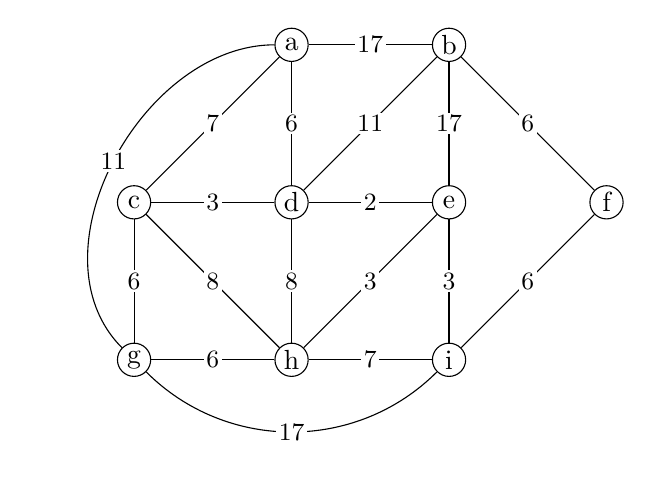
\begin{tikzpicture}
    \begin{scope}
        [vertex/.style={draw,circle,inner sep = 0em, minimum size = 1.2em},
        edgelabel/.style = {fill = white, inner sep = 0.1em, font=\small}]
       \node[vertex] (a) at (0,0) {a};
       \node[vertex] (b) at (2,0) {b};
       \node[vertex] (c) at (-2,-2) {c};
       \node[vertex] (d) at (0,-2) {d};
       \node[vertex] (e) at (2,-2) {e};
       \node[vertex] (f) at (4,-2) {f};
       \node[vertex] (g) at (-2,-4) {g};
       \node[vertex] (h) at (0,-4) {h};
       \node[vertex] (i) at (2,-4) {i};
       
       \draw[-] (a) to node[edgelabel] {$17$} (b);
       \draw[-] (a) to node[edgelabel] {$7$} (c);
       \draw[-] (a) to node[edgelabel] {$6$} (d);
       \draw[-, out = 180, in = 135] (a) to node[edgelabel] {$11$} (g);
       \draw[-] (b) to node[edgelabel] {$11$} (d);
       \draw[-] (b) to node[edgelabel] {$17$} (e);
       \draw[-] (b) to node[edgelabel] {$6$} (f);
       \draw[-] (c) to node[edgelabel] {$3$} (d);
       \draw[-] (c) to node[edgelabel] {$6$} (g);
       \draw[-] (c) to node[edgelabel] {$8$} (h);
       \draw[-] (d) to node[edgelabel] {$2$} (e);
       \draw[-] (d) to node[edgelabel] {$8$} (h);
       \draw[-] (e) to node[edgelabel] {$3$} (h);
       \draw[-] (e) to node[edgelabel] {$3$} (i);
       \draw[-] (f) to node[edgelabel] {$6$} (i);
       \draw[-] (g) to node[edgelabel] {$6$} (h);
       \draw[-, out = -45, in = -135] (g) to node[edgelabel] {$17$} (i);
       \draw[-] (h) to node[edgelabel] {$7$} (i);
    \end{scope}
    \end{tikzpicture}
    \end{document}